\documentclass[10pt]{standalone}
\usepackage{commands}

\begin{document}
    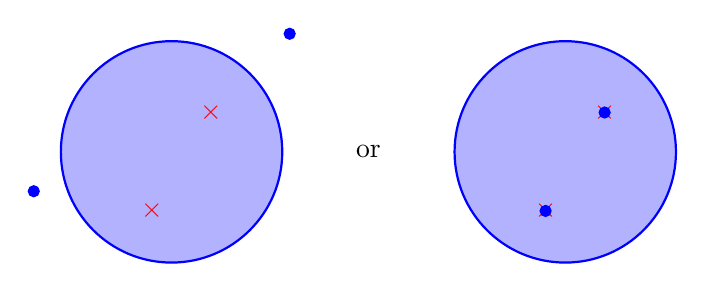
\begin{tikzpicture}
        \draw[blue, thick, fill = white!70!blue] (0, 0) circle (40pt);
        \node[red] at (0.5, 0.5) {$\times$};
        \node[red] at (-0.25, -0.75) {$\times$};
        \filldraw[blue, fill=blue] (1.5, 1.5) circle (2pt);
        \filldraw[blue, fill=blue] (-1.75, -0.5) circle (2pt);
        
        \node[] at (2.5, 0) {or};

        \draw[blue, thick, fill = white!70!blue] (5, 0) circle (40pt);
        \node[red] at (5.5, 0.5) {$\times$};
        \node[red] at (4.75, -0.75) {$\times$};
        \filldraw[blue, fill=blue] (5.5, 0.5) circle (2pt);
        \filldraw[blue, fill=blue] (4.75, -0.75) circle (2pt);
    \end{tikzpicture}
\end{document}